%!TEX root =  main.tex
\chapter{Implementation}\label{chapter:Implementation}
%
In this chapter, we are going to give more details about framework implemented based on formal model and architecture specification given i previous chapter.
Section~\ref{sec:framework} framework architecture, andd system implementation details. Section~\ref{sec:app} describe few possible senarios and applications that could utilize micro-clouds platform. In Section~\ref{sec:results} we present results of our experiments.
%
%
\section{Framework}\label{sec:framework}
%
We have implemented a proof of concept system based on the proposed, model using the microservice architecture with services that have distinct role and purpose to the entire system. These services are:

\begin{itemize}
	\item \textbf{Gateway}, this purpose is to export services feature to the rest of the world. Gateway is designed as a REST service, accepting $JSON$ style messages, so that various clients can communicate to the system. When request arrive at gateway, if request is valid it will pass request to the rest of the system. It communicate to rest of the services to check if user exists, does he have proper rights for actions that he send, and if not return proper message and do not propagete it to the rest of the system.
	\item \textbf{Authentification \& Authorization}, sole purpose of this service is to store users and their credentials. This servic will validate idoes user exists in the system, and does he have certen rights to performe some specific operation. Users that often use the system will be stored in the cache layer of the sevice, so that on next request his actions are done faster. Users that not use the system that often will not be stored in the cache, until first use. After that, if user do not use system in some time, he will expire from the cache.
	\item \textbf{Queues}, purpose of this service is to prevent huge request load to the system, and to accept more user requests. When user submit any \textbf{mutation} operation --- operation that change state of the system, thse opreations will be put in the queue. User can create their own queues, to prevent long lines for specific tasks. For example, user can crete queues for specific tasks, and use them only for those tasks, while other queues could be general purpos queues. On system start, evey user will start with one queue --- \textbf{default}. When doing mutations on different parts of the system, user can specify in matadata which queue he wnats task to go to.
	\item \textbf{Nodes}, this service stores and maintain informations about registered nodes in the system. All node hardware and software details will be stored in this here. This service is also responsabile for storeing metrics data, accept health-check requests from nodes, and inform rest of the system that used node is alive.
	\item \textbf{State}, is heart of the system. This service store all informations about architecture, clusters, regions and topologies. When new cluster/region/topology is creted, this service will setup watchers for nodes, so that if node is not send healtch-check signal for some time, that node will be declared dead. This is important, so that at any moment we must know state of the clusters and their utilization. This service as well will cache frequently used nodes data, so that on next request node lookup is faster since we can have huge number of nodes, topologies clusters and informations about them. To prevent data loss, this service will first store a copy of operation before attepting any mutation of the system.
	\item \textbf{Log}, is responsabile for storeing all log an trace data from every service. Here user can check are all jobs done, or is there some error and possible why error happend to resolve it, or fix for the next time. From user point of view, this is \textbf{read only} service and from sysem view this is \textbf{write only} service.
	\item \textbf{Command push}, purpose of this service is to push commands and operations to the nodes user desired. This service implement token bucket rate limiting algorithm to prevent constant data push to the nodes. As State service, this service will store a copy of operation information localy before attempting any push to the nodes. This information will be deleted, once operation reach all desided nodes, and all of them response with ACK message.
\end{itemize}

All services, are higly customizable and all have their own configuratoin file that could be changed and adopted. All these services are easy to extend to support new operations and informations about nodes, regions, clusters, topologies and latter on applications as well. 

The system operates with four commands, where three of them follow formal models described in previous chapter. Last command is simple command to list logs for every user.

In the rest of this section we will see details about all operations, as well as used technologies to implement whole system. We will describe possible applicatinos and give future directions for applicatoin development. System architecture is shown in Figure~\ref{fig:fig11}.

\begin{figure}[H]
	\begin{center}
		\includegraphics[scale=0.7]{images/FIG5}
	\end{center}
	\vspace{-0.9cm}
	\caption{Proof of concept implemented system.}
	\label{fig:fig11}
\end{figure}
%
%
\subsection{Technologies}\label{sec:technologies}
%
All services are implemented using the Go programming language, because his well-known tooling, support for developing system software, web based applications, small binaries but also great concurency model and ability to build binaries for almost any architecture without any changes in code. All services rely on go inplicit $interface$ implementation mechanism. Every technology or component used in the system can be swaped for some other, as long as that component implement $interface$ fully. Framework is developed in such a way that is relativly easy to extend, or switch and use different components and technologies.

As a main storage layer for our system, we used etcd, a popular open-source key-value database, that show good performance, and it is mostly used for configiration data. Metrics data are stored in the open-source time-series database InfluxDB. 

Communication between microservices is implemented in RPC manner using gRPC, and Protobuf as a message definition. gRPC and Protobuf are open-source tools designed by Google to be scalable, interoperable, and available for general purposes. Communication between nodes and the system is carried out using NATS, an open-source messaging system. Health checking and action push to nodes are implemented over NATS in a publish-subscribe manner.

Chacheing layer for every service is implemented using Redis key-value, in memory database. It is important to notice, that all concrete tools that are used, are easy swapable for some other as long as they implement proper interface.

All communication with the outside world, is done in REST manner using JSON encoded messages over HTTP. To communicate with the platform, we have developed a simple command-line interface (CLI) application also using the Go programming language that sends JSON encoded messages over HTTP to the system.

Every service is packed in a container, and for this purpose Docker containers are used. To achieve automatic orchestration, and self-heal and up-time, all services that are packed in containres, are runnin inside Kubernetes.

Every service will log details abot his usage and calls, as well as traces how requests are going. Log data is stored outside the service and container, and informations will be sent to centralized log storage on every $t$ seconds specified by user. Sending interval could be changed and addopted using configuration file for every service independently.

Log data will be stored in the two levels:

\begin{enumerate}[start=1,label={(\bfseries \arabic*)}]
	\item \textbf{system level}, this data is generated by the system, and could be viewd by administrators of the system \textbf{only}. Non operations people in the team or devops, but by developers of the system and providers of the system.
	\item \textbf{user level} that stores informations about user requests that \textbf{only} users can see. This type of data will not be visible to the developers of the system, and only users that created these logs will be able to see them.
\end{enumerate}

Log storage could be searched to see general state of the sytem, and informations about user requests and state of their requests.
%
%
\subsection{Node daemon}\label{sec:node_daemon}
Every node runs a simple daemon program implemented using the Go programming language, as an actor system (Ref. secion~\ref{sec:actor_model}). Actor system is developed for this purpose. When a message arrives, the proper actor will react based on the message type, or discard if the type is not supported. 

Extending such system is reather easy, because users need to simply write new actor and logic that goes with him and register it to the system.

When daemon start, he will first read configuration file to do proper setup, and then will contact actor system to start all the actors. 

System messages will be send to the daemon, but he will not react to these messages. Daemon is not able to communicate with any actor dyrectly. All communication goes trough actor system who is responsabile to pass messages to the actors. Actor system at this point have only tree existing actors:

\begin{enumerate}[start=1,label={(\bfseries \arabic*)}]
	\item \textbf{cluster actor}, this actor react on messages about new cluster formation, but he is also responsabile to contact rest of the system that message has arrived.
	\item \textbf{internal actor}, this actor react on messages from other actors in order to update daemon state. For example on new cluster creation, this actor will update daemon id, name, labels etc.
	\item \textbf{health actor}, this actor will periodicaly sent healtch-check data to the sytem about node state, utilization etc. This actor will communicate to the rest of the hardware to get proper informations, to collect logs from node and send all that data to the system.
\end{enumerate}

The actor system will monitor these actors, so in order that any of them crush for whatever reason, actor system will restart them. Listing~\ref{lst:listing3} show actor system hierarchy of existing actors.

\lstinputlisting[caption={Actor system hierarchy.}, label={lst:listing3}, captionpos=b, xleftmargin=.35\textwidth]{listings/listing3.txt}

Before daemon starts, the user needs to specify some parameters for proper configuration like: 

\begin{enumerate}[start=1,label={(\bfseries \arabic*)}]
	\item \textbf{identifier}
	\item \textbf{name}
	\item \textbf{labels}
	\item \textbf{health-check details}
	\item \textbf{system informations}
\end{enumerate} 

Configuration can be done easly using YAML configuration file. Listing~\ref{lst:listing1} show simple YAML configuration file for deamon process.

\lstinputlisting[caption={Daemon configiration file}, label={lst:listing1}, captionpos=b, xleftmargin=.35\textwidth]{listings/listing1.yaml}

Based on the configuration file, the daemon will start a background health-check mechanism, and it will subscribe to the system, using an identifier as a subscription topic. The background thread will contact the system repeatedly using a contact interval time, specified in the configuration file. 

On every health-check, the node will send labels, name, id, and metrics to the system (e.g., CPU utilization, total, used, free ram or disk, etc.). The specified labels will be used when the user is querying for available nodes, while node id will be used for reservation when forming a cluster.

On first start of the deamon when node is free, user can specify whathever node id he wants. Once, node is a part of the cluster, node id will be updated to match that. Node id update will happend on cluster formation process.
%\
%
\subsection{Mutate}\label{sec:mutate} 
Mutate operation (orange arrows in Figure \ref{fig:fig11}.) change the system state by creating, editing, or deleting clusters, regions, and topologies. When a user wants to perform a mutation over the system, a desired state needs to be specified using a YAML file. 

The users specify which nodes are forming the cluster. Optionally, users can also specify labels and names on the node level, and retention period on the cluster level. The retention period is used to describe how long metrics are going to be kept. When the retention period expires, the metrics data will be deleted or moved to another location. Users can target a specific system queue, by adding a metadata part in the configuration file. With this ability, users can have specific queues just for the mutation to avoid long waiting times if other queues are full. When forming a topology, users can assign a name and labels to the entire topology. These parameters will be used when the user wants to query all topologies to get full information about regions, clusters, and nodes inside a topology

\lstinputlisting[caption=Example of mutate file using YAML., label={lst:listing2}, captionpos=b, xleftmargin=.3\textwidth]{listings/listing2.yaml}
%
%
\subsection{List}\label{sec:list}  
This command show the current state of the system for the registered user (blue arrows in Figure \ref{fig:fig11}.). Using labels, the user can specify what part of the system he wants to see. He can get a global view of the system - all topologies he manages, or details about a single topology (i.e., regions, clusters, and nodes in a single topology). Users can specify a more detailed view of a single cluster, meaning the users will get information about what resources the cluster has, but also resource utilization over time (using stored metrics information); 
%
%
\subsection{Query}\label{sec:query} 
% 
This operation showing all or filtered free nodes registered to the system (yellow arrows in Figure \ref{fig:fig11}.). When a user wants to get information about free nodes, they need to submit a selector value which is composed of multiple key-value pairs. The selector will be used to compare labels of every free node existing in the system. The nodes satisfying the rules~\ref{frm:query_rule} defined in Section~\ref{sec:cluster_formation_protocol} will be in the result.

Querying process is little bit changed from one presented in Section~\ref{sec:cluster_formation_protocol}, and the only change is addition of the $Gateway$ service that will pass requests into the system and to prevent overflow of requests. This change \textbf{does not} affect or valiate formal model presented before.

Figure~\ref{fig:fig14} show communication diagram for query action.

\begin{figure}[H]
	\begin{center}
		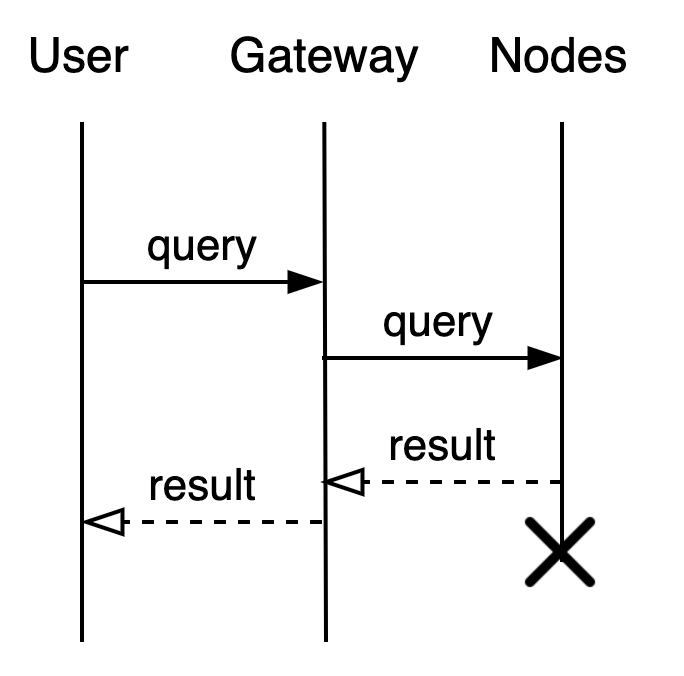
\includegraphics[scale=0.8]{images/Figure14}
	\end{center}
	\vspace{-0.7cm}
	\caption{Low level communication protocol diagram of query operation.}
	\label{fig:fig14}
\end{figure}
%
%
\subsection{Logs}\label{sec:logs}
% 
This operation showing stored logs and traces to the user (purple arrows in Figure \ref{fig:fig11}.). Here, the user can see the state of his operations and actions.
%
%
\section{Results}\label{sec:results} 
In our tests, we have used:

\begin{itemize}
	\item 9 Raspberry Pi 3+ Model B with 1GB LPDDR2 SDRAM, 16GB SDCard storage, and 1.4GHz Cortex-A53 64-bit SoC running Raspbian Linux, a Debian-based operating system.
	\item 3 Beagle bone black devices with 512MB DDR3 RAM, 4GB 8-bit eMMC on-board flash storage, and 1GHz ARM Cortex-A8 running a version of Linux Debian operating system.
\end{itemize}

\noindent
as test heterogenious nodes for creating clusters, regions, and topologies. 

Using Go tooling we were able to build daemon problam without changes and dissiminate on all nodes.

We have run tests on different configurations and different nodes clusters using these nodes. All nodes were connected on the WIFI network, and experiments were conducted in a controlled environment.

Experimental research was realized in the laboratory of the Department of Informatics at the Faculty of Technical Sciences in Novi Sad. The laboratory of the Department of Informatics is equipped with adequate computer, communication and software equipment on which the set goals in this thesis can be fully realized.
%
%
\section{Applications}\label{sec:app}
%
This research focus on a platform with geo-distributed edge nodes can be organized dynamically into the micro data-centers and regions based on the cloud model, but adapted for a different environment. This middle layer helps the power-hungry servers reduce traffic by serving the nearby population requests and possibly syncing their data without expensive consensus protocols [55]. These micro data-centers or micro clouds also increase the availability and reliability of the cloud services, and as such could be offered as a service to users.

With clear separation of concerns and a familiar application model for the users it opens possibilities for new human-centered applications, for example, area traffic control. 

If we imagine a scenario where a new catastrophic event (earthquake, tsunami, war, terrorist attack, pandemic, etc.) is in the human population, an increasing amount of ambulance vehicles must be routed to hospitals fast, in the city area for example. The traffic control system suddenly needs more resources to continue operating properly. On top of that, if the healthcare system is like the one presented in [56, 57], we can monitor patient health in real-time [58] and transfer data to the healthcare platform. 

This gives health workers crucial information about patients on their arrival. Resource vise, this scenario is relatively easy to solve if using the cloud, as we increase resource demand. The main advance of EC, when compared to the cloud only approach, is the acceleration of the communication speed. In our scenario, the cloud could bring huge latency, while EC originates from peer to peer systems [11], serving only local population needs, minimizing potentially huge round-trip time of the cloud. Furthermore, our model expands peer to peer systems into new directions and blends them with the cloud to allow novel human-centered, cloud-like applications. 

For applications like self-driving cars, delivery drones, or power balancing in electric grids require real-time processing for proper decision making, or any other application that future developers may develop.

Users are getting a new platform as a blank canvas, and there is no limitation in what applications they can develop. Integrating hardware and/or software even more, connecting sensors and things around us and eventually an operating system that will be capable of running city/state infrastructure without human intervention.
%
%